%02-ot-aiyenggar-discussion-paper.tex
\documentclass[12pt]{article}
\usepackage{amssymb,latexsym}
\usepackage[round,sort]{natbib}
\usepackage{multirow,array}
\usepackage{fancyhdr}
\usepackage{lastpage}
\usepackage{graphicx}
\usepackage[bottom]{footmisc}
\graphicspath{ {02-ot-aiyenggar-discussion-paper-images/} }
\usepackage[T1]{fontenc}
\usepackage{mathptmx}
\usepackage{tabu}
\usepackage{textcomp}
\usepackage{stata}
\usepackage{listings}
\usepackage{tikz} 
\usepackage{adjustbox}
\usepackage{longtable}
\usetikzlibrary{arrows,decorations.pathmorphing,backgrounds,fit,positioning,shapes.symbols,chains}
\newenvironment{hypothesis}{
  	\itshape
  	\leftskip=\parindent \rightskip=\parindent
  	\noindent\ignorespaces}
	
\pagestyle{fancy}
\fancyhf{}
\lhead{Readings on Structural Contingency Theory}
\rfoot{Page \thepage  \ of \pageref{LastPage}}
\rhead{Iyenggar}

\begin{document}
\title{Readings on Structural Contingency Theory:\\  Session 02 Organization Theory 2016}
\author{Ashwin Iyenggar  (1521001) \\ ashwin.iyenggar15@iimb.ernet.in} 


\maketitle
\thispagestyle{empty}


\abstract
In this discussion paper, we attempt to review structural contingency theory broadly. We then discuss the various perspectives from the assigned and additional readings for this session, and then lay out our interpretation\footnote{I am grateful to Prof. Abhoy Ojha for having suggested that the discussion paper be modeled along the lines of a literature review. } of the state of the literature, and of the strengths and weaknesses of the theory.


 \begin{quotation}
"The theory is scientific in style with the aim being to produce scientific knowledge of the type achieved in the natural sciences" \\ 
\null\hfill \textit{\cite{Donaldson1996a}, on Structural Contingency Theory}
 \end{quotation}
 
\section{Review of Structural Contingency Theory}\label{S:Review}
The primary construction in structural contingency theory is that the environment (e) causes a certain level of the contingency variable (c) which in turn causes the organization to adopt a certain structure (s). Therefore, e $\rightarrow$ c $\rightarrow$ s. Specifically, the degree of uncertainty (e) affects task uncertainty (c) which causes organizations to alter the degree of differentiation and integration (s) of their organizational structures \citep{Lawrence1967}. Task uncertainty may be either technical uncertainty or strategic uncertainty \citep{Whitley1984a}. Technical uncertainty is defined as the extent of variability in the methods accepted for empirical research in the area, while strategic uncertainty is defined as the extent to which there  are different views within the field, of which problems in the area are more important and which ones are less important and what goals should govern their research. It follows that higher the technical uncertainty or higher the strategic uncertainty, the more divergence one may observe in the area.

Following on the tenets of the structural contingency theory, a failure to conform to  the environment leads to reduced functionality for the organization. This then forces managers to adapt (note that this is a forced adaptation, not a voluntary adaptation).  \cite{Lawrence1967}  suggest that the optimal outcome is produced only by the organization structure that fits the contingency. Therefore from the perspective of contingency theory, the situation causes structure, and the ideas of the decision makers do not make a contribution in  explaining  the organization structure. 

Contingency also defines a state of fitness or fit when the firm is running efficiently. Firms that not operating under fitness are considered to be operating misfit. According to  contingency theory, firms are expected to monitor themselves for fit with the environment and to create organization structures that maximize fit. The theory expects that they perform this by the application of differentiation and integration routines \citep{Lawrence1967}, and by aligning strategy and structure of the organization so as to fit the environment. In summary therefore, organizational structure is explained by the need to fit contingencies.

Contingencies have been suggested as being any one of the following a) Environment \citep{Lawrence1967}, b) Internal Technology \citep{Woodward1965}, c) Organization Size \citep{Child1975,Khandwalla1973,Blau1970,Pugh1969}, and finally, d) Strategy \citep{Chandler1962}. The underlying philosophical assumption of the contingency theorists is that the phenomenon is governed by law-like relationships and that contingency factors can explain multiple dimensions of the organization structure.  Figure ~\ref{figure:sct} depicts how strong proponents of contingency theory view organizations in relation the their environments. The argument is that an environmental change cause a change in fit (misfit) that manifests itself as a change (a drop) in performance. The drop in performance leads to adaptation that should eventually reduce the extent of misfit, and thereby leading the firm toward fit.

\begin{figure}[h]
\centering
\begin{adjustbox}{width=\textwidth}
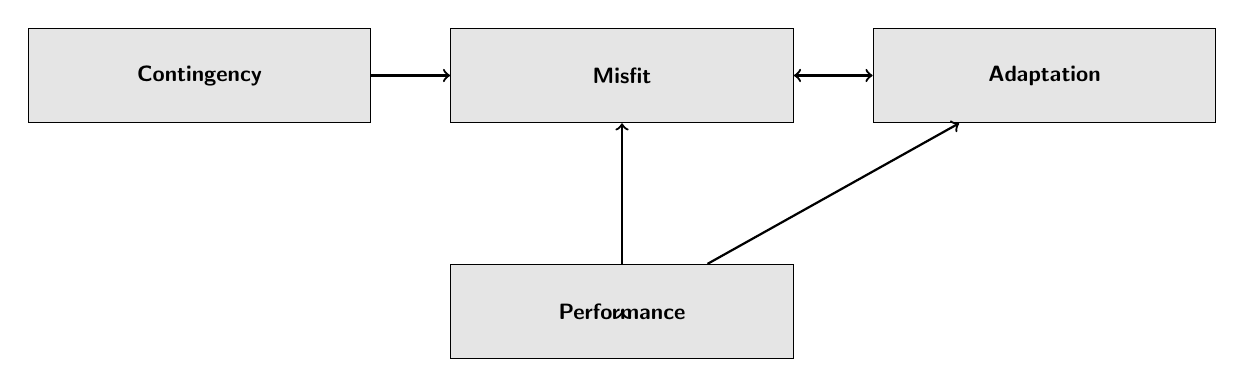
\begin{tikzpicture}
[node distance = 1cm, auto,font=\footnotesize,
every node/.style={node distance=3cm},
comment/.style={rectangle, inner sep= 5pt, text width=4cm, node distance=0.25cm, font=\scriptsize\sffamily},
force/.style={rectangle, draw, fill=black!10, inner sep=5pt, text width=4cm, text badly centered, minimum height=1.2cm, font=\bfseries\footnotesize\sffamily}] 

\node [force] (misfit) {Misfit};
\node [force, left=1cm of misfit] (contingency) {Contingency};
\node [force, right=1cm of misfit] (adaptation) {Adaptation};
\node [force, below of=misfit] (performance) {Performance};

\path[->,thick] 
(contingency) edge (misfit)
(performance) edge (misfit) edge
(performance) edge (adaptation);

\path[<->,thick] 
(misfit) edge (adaptation);

\end{tikzpicture} 
\end{adjustbox}
\caption{Relationships in Contingency Theory \citep{Donaldson1987}}
\label{figure:sct}
\end{figure}

When firms find themselves as misfit, the theory says that the firms make adaptive changes by adopting a new organization structure that bring them to fit \citep{Donaldson2001}. The fit between diversification and divisionalization is one example of a firm adapting to fit to meet with new circumstances \citep{Donaldson1987}. From the positivist point of view, structural contingency theory is similar to organizational economics in that organizations are seen as being molded by their situation. The functionist point of view focusses on the process by which the situation molds the organization, that manifests as adaptation and selection. While structural contingency theory is based on a positivist-functionist philosophical paradigm, many other theories in Organization Theory do not necessarily share the same philosophical moorings. Indeed several other theories build on other philosophical approaches like interpretist, conflict, critical, post modern, power or social action theories or social constructionism. Therefore, one way that this literature review could be positioned as, is as one of competing philosophical underpinnings.

\subsection{Breakaway Theories}
History bears  out  that after enjoying over 15 years of prominence as the dominant form of 'normal science' \citep{Kuhn1970} practiced in organization studies, structural contingency theory was challenged from inside as well as from outside. \cite{Knudsen2005} suggests that Organization Theory has since moved away from the bureaucratic structure during the hegemony of the structural contingency research program in the 1960\textquotesingle s and 1970\textquotesingle s to a polycentric oligarchy in the 1980\textquotesingle s due to the emergence of several new research programs. The arrival of the new theories such as population ecology, institutional theory, resource dependence theory, and transaction cost economics increased the task uncertainty and strategic uncertainty \citep{Whitley2000}. \cite{Knudsen2005} believes that the best structure to uphold balance of innovation and tradition is the polycentric oligarchy (we discussed this in session 01 and will not be discussed here further).

It is worth highlighting though that even in its prime,  structural contingency theory was unlike economics where the optimization paradigm offered economic theorists a coherent way of doing highly abstract theoretical work. Structural contingency theory had become a program for standardizing empirical research and testing empirical structure-contingency relationships than for solving theoretical problems. While the optimization paradigm had reduced strategic task uncertainty for economics,  structural contingency theory had reduced technical task uncertainty  and could not separate the theoretical puzzle solving from empirical research. 


\section{Critical Analysis of Assigned Readings}
Table ~\ref{table:themes}  lists the articles that were reviewed for this discussion paper. Apart from \cite{Donaldson1987}, each of them highlights a problematic area for structural contingency theory.

\begin{center}
\begin{longtable}{|p{0.2\textwidth}|p{0.4\textwidth}|p{0.3\textwidth}|}
\label{table:themes}\\
\hline \textbf{Article}&\textbf{Key Idea of Study}&\textbf{Key Constructs in Study}\\\hline
\endfirsthead
\hline \textbf{Article}&\textbf{Key Idea of Study}&\textbf{Key Constructs in Study}\\\hline
\endhead

\cite{Donaldson1987}&Structural Adjustment to Regain Fit is adequate to support a dynamic view of contingency theory&Contingency, Misfit, Performance, Adjustment\\\hline
\cite{Smith2011}&Simultaneous responses to paradoxical tensions to achieve short-term peak performance that fuels long term performance&Latent Tensions, Salient Tensions, Acceptance, Paradoxical Resolution, Sustainability\\\hline
\cite{Menz2014}&Adaptation does not significantly affect firm financial performance&Strategic and Structural Complexity, Adaptation, Performance\\\hline
\cite{Siggelkow2002}&Organizations transition between configurations by four paths&Thickening, Patching, Coasting or Trimming\\\hline
\cite{Payne2006}&Suboptimal equifinality and trade-off equifinality are more common than instances of true contingency theory&Organizational Configuration, Financial Performance\\\hline
\cite{Miller1992}&Internal fit and external fit often, but not always are inconsistent with each other. &Environmental uncertainty, Environmental diversity, Formalization, Centralization, Specialization\\\hline
\cite{Sillince2005}&Rhetoric congruence is a necessary condition for contingency theory to hold&Emphasizing Context, Switching Perspective, Creating Consistency, Creating Purpose, Differentiation and Integration Rhetoric\\\hline
\cite{Ethiraj2004}&Organization hierarchy is a key determinant of effectiveness of organization&Hierarchy loosely coupled, Hierarchy non-loosely coupled, First-order Adaptation, Second-order Adaptation\\\hline
\cite{Moon2004}&Contingency Theory requires a Dynamic Logic that challenges the assumption of symmetric adaptation&Nature of Structural Adaptation, Task Environment, Cognitive Ability, Team coordination, Team Performance\\\hline
\cite{Short2008}&Organizational configuration offers potential for further understanding organizations and strategy&Configuration, Performance\\\hline
\caption {Synopsis of Readings in Structural Contingency Theory}
\end{longtable}
\end{center}

While \cite{Donaldson1987} is the strongest proponent for contingency theory in the above, \cite{Smith2011} argue for an alternate model to also co-exist. While \cite{Menz2014} raise the question if adaptation really contributes to fit, \cite{Siggelkow2002} suggests that the process of adaptation is open to multiple possibilities. \cite{Miller1992} raises the point that organizations are often fraught with inconsistencies between internal and external constituents, while \cite{Ethiraj2004} argue that adaptation levels are influenced by organization hierarchy. It is clear in each of the works outside of \cite{Donaldson1987} that the case for contingency theory is weakened, and that it may at best be valid in an extremely narrow context. In the following sections, I lay out my view on the issues raised by considering a series of questions. I will summarize them in the discussion session following these.

\subsection{Static Theory or Dynamic Theory?}
\cite{Donaldson1987} identifies that the primary criticism of structural contingency theory is that is static. He addresses this issue by suggesting that including the link from misfit to performance and that from performance to adaptation addresses the static concern and makes his neo-contingency theory effective. The static theory criticism however goes much deeper than how \cite{Donaldson1987} believes it to be. First, not only are the firm and the environment each undergoing simultaneous change, but their underlying components and agents may also each be undergoing change at a different rate. Unless this dynamism is adequately captured in the theory, it would be inappropriate to accept the argument forwarded by \cite{Donaldson1987}. \cite{Smith2011} capture the dynamics involved in the process of organization change better, and their proposition that there maybe a need for a cyclically adjusted response that achieves short-term peak performance that fuels long term performance is on much firmer ground. However, in capturing the dynamics of the phenomenon, one must also recognize and account for a) there being unintended consequences, and b) for there to be emergent effects. Both the above ideas come from the complex-adaptive systems literature, and is something that has not been explicitly captured by any of the articles reviewed. 

\subsection{Paradox or Straightjacket?}
While \cite{Smith2011} make a good case for disparate and divergent aspects to be modeled together rather than for one to be assumed away. However, as \cite{Miller1992} demonstrates, organizations are not always faced with paradoxical choices. Therefore the framework must allow for paradoxes to surface where they are indeed in conflict, but also recognize that they may in many cases not conflict in the specific application organization change. 

\subsection{Equilibrium Study or Process Study?}
Economic theory has been heavily influenced by the paradigm of equilibrium where the transformation from cause to effect is assumed to be automatic and atomic. However, as pointed out eloquently in the single case study on Vanguard in \cite{Siggelkow2002}, firms have the option of choosing between patching or thickening, and between coasting and thinning. Additionally these processes themselves are influenced by the larger direction of change. Thus a punctuated equilibrium approach would have the organization making different choices than in a thin-to-thick approach. Given that organization configurations do not transition in straight jacketed ways, the importance of rich process studies to understand the nuances of change cannot to overemphasized. The criticism of the contingency theory is therefore that in attempting an equilibrium driven specification, that the theory is straying far away from the phenomenon that it is trying to study.

\subsection{Definition of Fit}
Many of the constructs in contingency theory strike at the problem of ambiguity of specification. The notion of fit, for example is one that is highly subjective and therefore problematic. While the challenges involved in quantifying complex organizations and their processes is not lost on me, the attempt for contingency theory to hold on to the strong paradigm model when the underlying constructs were themselves so tenuous, definitely warrants criticism. Organization scholars are better served when they model their phenomena on the basis of the underlying nature of the phenomena than when theories are held strong so as to fit a  definition of scientific rigor that while appropriate in the natural sciences, is not quite relevant in organizational studies.


\subsection{Does Internal Fit Matter?}
\cite{Miller1992} and \cite{Smith2011} both articulate well the role of internal organizational processes and agents in the adaptation of the firm. Clearly this is one huge hole in contingency's treatment of the issue of organizational change. A more realistic model of organizational change must include both internal fit as well as external fit. However, I would suggest that the internal-external interaction be moderated by firm-boundaries and intra-firm boundaries so as to both keep the complexity of the model in check as well as to align it to the realities of the phenomenon.

\subsection{Does misfit always lead to fit?}
A startling assumption in contingency theory is that on recognition of misfit and lower performance, that managers would undertake adaptation toward fit. However as \cite{Payne2006} points out, realistic situations may not quite allow for managers to know this. As \cite{Siggelkow2002} points out, even Vanguard had a few instances where misfits had to eventually be abandoned. In this light, the finding by \cite{Menz2014} that CSO presence did not affect financial performance is not that surprising at all. We therefore suggest that this strong assumption that misfit automatically leads to actions toward fit be nuanced and multiple outcomes be allowed.

\subsection{Notion of Time}
Multiple studies including \cite{Siggelkow2002} and \cite{Smith2011} point to the importance of time in modeling organizational phenomena. We suggest that this is a dimension that has been heavily been overlooked in favour of more tractable and parsimonious construction of theory. Specifically the notion of time applies in two forms: First, as evidenced in Vanguard study \citep{Siggelkow2002}, patching is a frequent approach by which organizations evolve. Patching is both path dependent and a function of the environment at a particular time. Equally, after a certain stage the processes seem adequately thickened so that time factors affect organization processes less. Second, as highlighted by \cite{Smith2011}, firms are concerned with both short term peak performance, but also long term performance and survival. Contingency theory's single notion of fit therefore becomes a constraint imposed by the theory that may not be true in reality. More realistic representations of organization change must therefore accommodate multiple time-period objectives.

\subsection{Dissemination to Practioners}
As scholars of an applied area with direct relevance to practice, the question that comes up is that our theories do eventually have to be able to be disseminated in ways that practitioners may be able to apply it to organization issues they face. While on the one hard contingency theory was simple and therefore could be easily disseminated and practiced. However as this theory is less and less useful to practice, one may be tempted to disseminate a full blown complex theory that captures all nature of interconnections. However this may have the affect of turning off practitioners from using any academic theory. We must therefore strive to build specific actionable models that are empirically valid, but nevertheless falsifiable.

\subsection{Why Contingency Theory Stays On?}
We note that normal science progresses \cite{Kuhn1970}, contingency theory lives on as neo-contingency theory. Though significantly weakened by the various contradictions, the single biggest factor seems to me that a dominant paradigm that is not falsifiable may be very hard to overthrow. Proponents would always argue that while the theory may not quite hold in a specific environment, that it is generally a useful construction of the phenomenon. And since contingency theory is neither falsifiable, nor is subsumable into other theories due to philosophical contradictions, it lives on as one of many other theories in organization theory.

\section{Discussion}
As evidenced by our positions in each of the questions above, our position is one for capturing the dynamics of the phenomena as truly as possible without the weight of a dominant paradigm overbearing on what the theory should be. Therefore, while we argue that the environment does not necessarily have to drive organization change all the time, but that it may go both ways. We therefore model both internal agents and external agents to be captured  richly in the theory of organization change. We also note  simultaneously  that not all agents affect all outcomes all the time. We suggest that the notion of simultaneity is appropriate \citep{Smith2011} as is the notion of agents navigating between a few set of well defined processes \citep{Siggelkow2002}. We argue for time to be integrated as an essential construct both from allowing organizational states to be defined in terms of time, but also for organization outcomes to be set on multiple time horizons. Our conception of organization change is that of a complex adaptive system where each of agents may be modeled in local environments, but where interaction effects lead to emergent properties that may not be able to be captured by simple parsimonious theory as contingency theory.


\bibliography{/Users/aiyenggar/OneDrive/code/bibliography/ae,/Users/aiyenggar/OneDrive/code/bibliography/fj,/Users/aiyenggar/OneDrive/code/bibliography/ko,/Users/aiyenggar/OneDrive/code/bibliography/pt,/Users/aiyenggar/OneDrive/code/bibliography/uz} 
\bibliographystyle{apalike}

\end{document}
